%-*-latex-*-
% https://en.wikipedia.org/wiki/Heapsort#Variations

\sectionthree{Heapsort}
\begin{python0}
from solutions import *; clear()
\end{python0}

\textsc{Heapsort given a maxheap.}
Now we delete the root from the heap.
Because this is a maxheap, the root, is the 
maximum value of \verb!x[0..9]!.
We swap \verb!x[0]! and \verb!x[9]!
and re-heapify to get a heap \verb!x[0..8]!.
In other words we're essentially doing a delete of the value at \verb!x[0]!
(the extract-max operation), putting this value at \texttt{x[9]}.

We repeat the above to get a heap \verb!x[0..7]!.
At this point the largest value of the array is at \verb!x[9]!
and the second largest is at \verb!x[8]!.

We repeat until the heap has only one value, i.e., the heap is \verb!x[0]!.
The whole array must be sorted in ascending order.

The runtime is, informally, $\log_2 n + \log_2 (n - 1) + \cdots$
which is $\log_2 n! \leq \log_2 n^n = n \log_2 n$.

So the total time for the above process,
creating the heap and then removing roots from the 
heap is roughly $2 n \log_2 n$ and therefore
the runtime for heapsort is $O(n \log_2 n)$.

Note that the heapsort has a worse runtime of $n \log_2 n$
whereas quicksort can have a worse runtime of $n^2$
although
on the average quicksort is $O(n \log n)$ and 
typically quicksort is faster than heapsort by a constant
factor.
Although mergesort does achieve $n \log_2 n$ for worse runtime,
remember that mergesort needs $O(n)$ space.
However heapsort is not stable whereas mergesort is stable.


\begin{ex} 
  \label{ex:some-decision1}
  \tinysidebar{\debug{exercises/{empty0/question.tex}}}
  \solutionlink{sol:some-decision1}
  \qed
\end{ex} 
\begin{python0}
from solutions import *
add(label="ex:some-decision1",
    srcfilename='exercises/some-decision1/answer.tex') 
\end{python0}


\newpage
Here is a maxheap say constructed
using build-maxheap:


\begin{center}

\begin{tikzpicture}
\node at (4,-0.8) [minimum size=8mm] (Z) {$$};
\node at (2,-1.6) [circle,draw,minimum size=8mm] (A) {$\beta$};
\node at (0,-2.4000000000000004)
    [isosceles triangle, shape border rotate=+90,
     draw,minimum size=8mm,minimum height=2cm,
     anchor=north] (Ctriangle) {$T_1$};
\coordinate (C) at (0,-2.4000000000000004);
\node at (4,-2.4000000000000004) [circle,draw,minimum size=8mm] (B) {$\alpha$};
\node at (3,-3.2)
    [isosceles triangle, shape border rotate=+90,
     draw,minimum size=8mm,minimum height=2cm,
     anchor=north] (Dtriangle) {$T_2$};
\coordinate (D) at (3,-3.2);
\node at (5,-3.2)
    [isosceles triangle, shape border rotate=+90,
     draw,minimum size=8mm,minimum height=2cm,
     anchor=north] (Etriangle) {$T_3$};
\coordinate (E) at (5,-3.2);
\draw [-,thick] (Z) -- (A);
\draw [-,thick] (A) -- (B);
\draw [-,thick] (A) -- (C);
\draw [-,thick] (B) -- (D);
\draw [-,thick] (B) -- (E);

;
\end{tikzpicture}
    
\end{center}


Let's perform heapsort on this maxheap.
Recall that extract-root will throw away the root by replacing
the value at the root with the last value in the tree (i.e.,
the rightmost value at the last level of the tree).
Instead of replacing the root with the last value,
I will \textit{swap} the root value and last value.
Otherwise it's the same extract-root operation.
Let's do it.


\textsc{Step 1}.
First I swap the root value and the last value:

\input{stdout63.tex}


I color \texttt{9} in red to remind myself
that the \texttt{9} should not be considered part of the maxheap,
but of course it's in the array.
In terms of an array the above diagram would correspond to this array:

\begin{center}
\begin{tikzpicture}

\fill[white] (5.0, 0.0) circle (0.3);
\node [draw=none,line width=0cm,black,minimum size=0.6cm,circle] at (5.0,0.0)(X){};
\fill[white] (17.0, 0.0) circle (0.3);
\node [draw=none,line width=0cm,black,minimum size=0.6cm,circle] at (17.0,0.0)(Y){};
\fill[white] (11.0, 0.0) circle (0.3);
\node [line width=0.03cm,black,minimum size=0.57cm,draw,circle] at (11.0,0.0)(a){};\draw (11.0, 0.0) node[color=black] {\texttt{18}};
\fill[white] (9.0, -1.0) circle (0.3);
\node [line width=0.03cm,black,minimum size=0.57cm,draw,circle] at (9.0,-1.0)(b){};\draw (9.0, -1.0) node[color=black] {\texttt{10}};
\fill[white] (14.0, -2.0) circle (0.3);
\node [line width=0.03cm,black,minimum size=0.57cm,draw,circle] at (14.0,-2.0)(d){};\draw (14.0, -2.0) node[color=black] {\texttt{20}};
\fill[white] (8.0, -2.0) circle (0.3);
\node [line width=0.03cm,black,minimum size=0.57cm,draw,circle] at (8.0,-2.0)(e){};\draw (8.0, -2.0) node[color=black] {\texttt{4}};
\fill[white] (12.0, -2.0) circle (0.3);
\node [line width=0.03cm,black,minimum size=0.57cm,draw,circle] at (12.0,-2.0)(f){};\draw (12.0, -2.0) node[color=black] {\texttt{19}};
\fill[white] (8.0, -4.0) circle (0.3);
\node [line width=0.03cm,black,minimum size=0.57cm,draw,circle] at (8.0,-4.0)(k){};\draw (8.0, -4.0) node[color=black] {\texttt{3}};
\fill[white] (7.0, -3.0) circle (0.3);
\node [line width=0.03cm,black,minimum size=0.57cm,draw,circle] at (7.0,-3.0)(l){};\draw (7.0, -3.0) node[color=black] {\texttt{2}};
\fill[white] (13.0, -1.0) circle (0.3);
\node [line width=0.03cm,black,minimum size=0.57cm,draw,circle] at (13.0,-1.0)(p){};\draw (13.0, -1.0) node[color=black] {\texttt{26}};
\fill[white] (6.0, -4.0) circle (0.3);
\node [line width=0.03cm,black,minimum size=0.57cm,draw,circle] at (6.0,-4.0)(n){};\draw (6.0, -4.0) node[color=black] {\texttt{0}};
\fill[white] (10.0, -2.0) circle (0.3);
\node [line width=0.03cm,black,minimum size=0.57cm,draw,circle] at (10.0,-2.0)(q){};\draw (10.0, -2.0) node[color=black] {\texttt{17}};\draw[line width=0.03cm,black,->,>=triangle 60] (e) to  (l);
\draw[line width=0.03cm,black,->,>=triangle 60] (p) to  (d);
\draw[line width=0.03cm,black,->,>=triangle 60] (b) to  (q);
\draw[line width=0.03cm,black,->,>=triangle 60] (l) to  (n);
\draw[line width=0.03cm,black,->,>=triangle 60] (l) to  (k);
\draw[line width=0.03cm,black,->,>=triangle 60] (p) to  (f);
\draw[line width=0.03cm,black,->,>=triangle 60] (a) to  (p);
\draw[line width=0.03cm,black,->,>=triangle 60] (a) to  (b);
\draw[line width=0.03cm,black,->,>=triangle 60] (b) to  (e);
\end{tikzpicture}

\end{center}



I still need to heapify-down the \texttt{6} to get this:

\begin{center}
\begin{tikzpicture}

\fill[white] (5.0, 0.0) circle (0.3);
\node [draw=none,line width=0cm,black,minimum size=0.6cm,circle] at (5.0,0.0)(X){};
\fill[white] (17.0, 0.0) circle (0.3);
\node [draw=none,line width=0cm,black,minimum size=0.6cm,circle] at (17.0,0.0)(Y){};
\fill[white] (13.0, -1.0) circle (0.3);
\node [line width=0.03cm,black,minimum size=0.57cm,draw,circle] at (13.0,-1.0)(a){};\draw (13.0, -1.0) node[color=black] {\texttt{10}};
\fill[white] (11.0, 0.0) circle (0.3);
\node [line width=0.03cm,black,minimum size=0.57cm,draw,circle] at (11.0,0.0)(b){};\draw (11.0, 0.0) node[color=black] {\texttt{4}};
\fill[white] (15.0, -3.0) circle (0.3);
\node [line width=0.03cm,black,minimum size=0.57cm,draw,circle] at (15.0,-3.0)(d){};\draw (15.0, -3.0) node[color=black] {\texttt{20}};
\fill[white] (9.0, -1.0) circle (0.3);
\node [line width=0.03cm,black,minimum size=0.57cm,draw,circle] at (9.0,-1.0)(e){};\draw (9.0, -1.0) node[color=black] {\texttt{2}};
\fill[white] (13.0, -3.0) circle (0.3);
\node [line width=0.03cm,black,minimum size=0.57cm,draw,circle] at (13.0,-3.0)(f){};\draw (13.0, -3.0) node[color=black] {\texttt{17}};
\fill[white] (8.0, -2.0) circle (0.3);
\node [line width=0.03cm,black,minimum size=0.57cm,draw,circle] at (8.0,-2.0)(k){};\draw (8.0, -2.0) node[color=black] {\texttt{0}};
\fill[white] (10.0, -2.0) circle (0.3);
\node [line width=0.03cm,black,minimum size=0.57cm,draw,circle] at (10.0,-2.0)(l){};\draw (10.0, -2.0) node[color=black] {\texttt{3}};
\fill[white] (14.0, -2.0) circle (0.3);
\node [line width=0.03cm,black,minimum size=0.57cm,draw,circle] at (14.0,-2.0)(p){};\draw (14.0, -2.0) node[color=black] {\texttt{18}};
\fill[white] (14.0, -4.0) circle (0.3);
\node [line width=0.03cm,black,minimum size=0.57cm,draw,circle] at (14.0,-4.0)(h){};\draw (14.0, -4.0) node[color=black] {\texttt{19}};
\fill[white] (16.0, -4.0) circle (0.3);
\node [line width=0.03cm,black,minimum size=0.57cm,draw,circle] at (16.0,-4.0)(m){};\draw (16.0, -4.0) node[color=black] {\texttt{26}};\draw[line width=0.03cm,black,->,>=triangle 60] (b) to  (a);
\draw[line width=0.03cm,black,->,>=triangle 60] (p) to  (f);
\draw[line width=0.03cm,black,->,>=triangle 60] (p) to  (d);
\draw[line width=0.03cm,black,->,>=triangle 60] (a) to  (p);
\draw[line width=0.03cm,black,->,>=triangle 60] (b) to  (e);
\draw[line width=0.03cm,black,->,>=triangle 60] (e) to  (k);
\draw[line width=0.03cm,black,->,>=triangle 60] (e) to  (l);
\draw[line width=0.03cm,black,->,>=triangle 60] (d) to  (h);
\draw[line width=0.03cm,black,->,>=triangle 60] (d) to  (m);
\end{tikzpicture}

\end{center}


\input{stdout66.tex}

Because I started with a maxheap, \verb!9!, the value I get from extract-root,
is the largest value in the array.
Since it moved to the last index position in the array,
this means that \verb!9! has found its right place.


\textsc{Step 2}.
Now I repeat the above process:
first I swap the root (i.e., \texttt{8}) and
the last value of the tree (i.e., \texttt{0}) to get this:


\begin{center}
\begin{tikzpicture}

\fill[white] (0.0, 0.0) circle (0.3);
\node [line width=0.03cm,black,minimum size=0.57cm,draw,circle] at (0.0,0.0)(14){};\draw (0.0, 0.0) node[color=black] {\texttt{14}};
\fill[white] (-3.2, -1.0) circle (0.3);
\node [line width=0.03cm,black,minimum size=0.57cm,draw,circle] at (-3.2,-1.0)(9){};\draw (-3.2, -1.0) node[color=black] {\texttt{9}};
\fill[white] (3.2, -1.0) circle (0.3);
\node [line width=0.03cm,black,minimum size=0.57cm,draw,circle] at (3.2,-1.0)(18){};\draw (3.2, -1.0) node[color=black] {\texttt{18}};
\fill[white] (-4.8, -2.0) circle (0.3);
\node [line width=0.03cm,black,minimum size=0.57cm,draw,circle] at (-4.8,-2.0)(5){};\draw (-4.8, -2.0) node[color=black] {\texttt{5}};
\fill[white] (-1.6, -2.0) circle (0.3);
\node [line width=0.03cm,black,minimum size=0.57cm,draw,circle] at (-1.6,-2.0)(13){};\draw (-1.6, -2.0) node[color=black] {\texttt{13}};
\fill[white] (1.6, -2.0) circle (0.3);
\node [line width=0.03cm,black,minimum size=0.57cm,draw,circle] at (1.6,-2.0)(15){};\draw (1.6, -2.0) node[color=black] {\texttt{15}};
\fill[white] (4.8, -2.0) circle (0.3);
\node [line width=0.03cm,black,minimum size=0.57cm,draw,circle] at (4.8,-2.0)(22){};\draw (4.8, -2.0) node[color=black] {\texttt{22}};
\fill[white] (-5.6, -3.0) circle (0.3);
\node [line width=0.03cm,black,minimum size=0.57cm,draw,circle] at (-5.6,-3.0)(0){};\draw (-5.6, -3.0) node[color=black] {\texttt{0}};
\fill[white] (-4.0, -3.0) circle (0.3);
\node [line width=0.03cm,black,minimum size=0.57cm,draw,circle] at (-4.0,-3.0)(8){};\draw (-4.0, -3.0) node[color=black] {\texttt{8}};
\fill[white] (-2.4, -3.0) circle (0.3);
\node [line width=0.03cm,black,minimum size=0.57cm,draw,circle] at (-2.4,-3.0)(10){};\draw (-2.4, -3.0) node[color=black] {\texttt{10}};
\fill[white] (4.0, -3.0) circle (0.3);
\node [line width=0.03cm,black,minimum size=0.57cm,draw,circle] at (4.0,-3.0)(21){};\draw (4.0, -3.0) node[color=black] {\texttt{21}};
\fill[white] (5.6, -3.0) circle (0.3);
\node [line width=0.03cm,black,minimum size=0.57cm,draw,circle] at (5.6,-3.0)(31){};\draw (5.6, -3.0) node[color=black] {\texttt{31}};
\fill[white] (-4.4, -4.0) circle (0.3);
\node [line width=0.03cm,black,minimum size=0.57cm,draw,circle] at (-4.4,-4.0)(7){};\draw (-4.4, -4.0) node[color=black] {\texttt{7}};
\fill[white] (-2.0, -4.0) circle (0.3);
\node [line width=0.03cm,black,minimum size=0.57cm,draw,circle] at (-2.0,-4.0)(11){};\draw (-2.0, -4.0) node[color=black] {\texttt{11}};
\fill[white] (3.6, -4.0) circle (0.3);
\node [line width=0.03cm,black,minimum size=0.57cm,draw,circle] at (3.6,-4.0)(19){};\draw (3.6, -4.0) node[color=black] {\texttt{19}};\draw[line width=0.03cm,black,->,>=triangle 60] (14) to  (9);
\draw[line width=0.03cm,black,->,>=triangle 60] (14) to  (18);
\draw[line width=0.03cm,black,->,>=triangle 60] (9) to  (5);
\draw[line width=0.03cm,black,->,>=triangle 60] (9) to  (13);
\draw[line width=0.03cm,black,->,>=triangle 60] (18) to  (15);
\draw[line width=0.03cm,black,->,>=triangle 60] (18) to  (22);
\draw[line width=0.03cm,black,->,>=triangle 60] (5) to  (0);
\draw[line width=0.03cm,black,->,>=triangle 60] (5) to  (8);
\draw[line width=0.03cm,black,->,>=triangle 60] (13) to  (10);
\draw[line width=0.03cm,black,->,>=triangle 60] (22) to  (21);
\draw[line width=0.03cm,black,->,>=triangle 60] (22) to  (31);
\draw[line width=0.03cm,black,->,>=triangle 60] (8) to  (7);
\draw[line width=0.03cm,black,->,>=triangle 60] (10) to  (11);
\draw[line width=0.03cm,black,->,>=triangle 60] (21) to  (19);
\end{tikzpicture}

\end{center}


\begin{center}
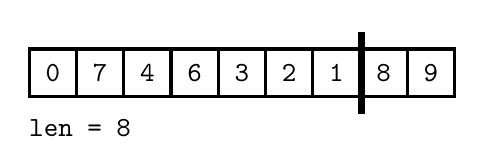
\begin{tikzpicture}

\draw (0.3, -0.3)
  node[draw, line width=0.04cm, , color=black,
       rounded corners=0cm, inner sep=0cm] {

\begin{minipage}[t][0.6cm]{0.6cm}
\mbox{}

\end{minipage}

};\draw (0.3, -0.3) node[color=black] {{\texttt{0}}};
\draw (0.8999999999999999, -0.3)
  node[draw, line width=0.04cm, , color=black,
       rounded corners=0cm, inner sep=0cm] {

\begin{minipage}[t][0.6cm]{0.6cm}
\mbox{}

\end{minipage}

};\draw (0.8999999999999999, -0.3) node[color=black] {{\texttt{7}}};
\draw (1.5, -0.3)
  node[draw, line width=0.04cm, , color=black,
       rounded corners=0cm, inner sep=0cm] {

\begin{minipage}[t][0.6cm]{0.6cm}
\mbox{}

\end{minipage}

};\draw (1.5, -0.3) node[color=black] {{\texttt{4}}};
\draw (2.0999999999999996, -0.3)
  node[draw, line width=0.04cm, , color=black,
       rounded corners=0cm, inner sep=0cm] {

\begin{minipage}[t][0.6cm]{0.6cm}
\mbox{}

\end{minipage}

};\draw (2.0999999999999996, -0.3) node[color=black] {{\texttt{6}}};
\draw (2.7, -0.3)
  node[draw, line width=0.04cm, , color=black,
       rounded corners=0cm, inner sep=0cm] {

\begin{minipage}[t][0.6cm]{0.6cm}
\mbox{}

\end{minipage}

};\draw (2.7, -0.3) node[color=black] {{\texttt{3}}};
\draw (3.3, -0.3)
  node[draw, line width=0.04cm, , color=black,
       rounded corners=0cm, inner sep=0cm] {

\begin{minipage}[t][0.6cm]{0.6cm}
\mbox{}

\end{minipage}

};\draw (3.3, -0.3) node[color=black] {{\texttt{2}}};
\draw (3.9, -0.3)
  node[draw, line width=0.04cm, , color=black,
       rounded corners=0cm, inner sep=0cm] {

\begin{minipage}[t][0.6cm]{0.6cm}
\mbox{}

\end{minipage}

};\draw (3.9, -0.3) node[color=black] {{\texttt{1}}};
\draw (4.5, -0.3)
  node[draw, line width=0.04cm, , color=black,
       rounded corners=0cm, inner sep=0cm] {

\begin{minipage}[t][0.6cm]{0.6cm}
\mbox{}

\end{minipage}

};\draw (4.5, -0.3) node[color=black] {{\texttt{8}}};
\draw (5.1, -0.3)
  node[draw, line width=0.04cm, , color=black,
       rounded corners=0cm, inner sep=0cm] {

\begin{minipage}[t][0.6cm]{0.6cm}
\mbox{}

\end{minipage}

};\draw (5.1, -0.3) node[color=black] {{\texttt{9}}};\draw[line width=0.1cm,black] (4.22,-0.82) to  (4.22,0.22);

\draw (1.0, -1.0)
  node[draw=none, line width=0cm, , color=black,
       rounded corners=0cm, inner sep=0cm] {

\begin{minipage}[t][0.1cm]{2cm}
\mbox{}

\end{minipage}

};
\draw (1.0, -1.0) node[color=black,
 inner sep=0cm] {
 
\begin{minipage}[t][0.1cm]{2cm}
\texttt{len = 8}
\end{minipage}

};
\end{tikzpicture}

\end{center}



(at this point \verb!9! and \verb!8! are not part of the heap)
then I heapify-down \texttt{0} to get this:

\begin{center}
\begin{tikzpicture}

\fill[white] (0.0, 0.0) circle (0.3);
\node [line width=0.03cm,black,minimum size=0.57cm,draw,circle] at (0.0,0.0)(10){};\draw (0.0, 0.0) node[color=black] {\texttt{10}};
\fill[white] (-3.0, -1.0) circle (0.3);
\node [line width=0.03cm,black,minimum size=0.57cm,draw,circle] at (-3.0,-1.0)(2){};\draw (-3.0, -1.0) node[color=black] {\texttt{2}};
\fill[white] (3.0, -1.0) circle (0.3);
\node [line width=0.03cm,black,minimum size=0.57cm,draw,circle] at (3.0,-1.0)(18){};\draw (3.0, -1.0) node[color=black] {\texttt{18}};
\fill[white] (-4.5, -2.0) circle (0.3);
\node [line width=0.03cm,black,minimum size=0.57cm,draw,circle] at (-4.5,-2.0)(0){};\draw (-4.5, -2.0) node[color=black] {\texttt{0}};
\fill[white] (-1.5, -2.0) circle (0.3);
\node [line width=0.03cm,black,minimum size=0.57cm,draw,circle] at (-1.5,-2.0)(4){};\draw (-1.5, -2.0) node[color=black] {\texttt{4}};
\fill[white] (1.5, -2.0) circle (0.3);
\node [line width=0.03cm,black,minimum size=0.57cm,draw,circle] at (1.5,-2.0)(17){};\draw (1.5, -2.0) node[color=black] {\texttt{17}};
\fill[white] (4.5, -2.0) circle (0.3);
\node [line width=0.03cm,black,minimum size=0.57cm,draw,circle] at (4.5,-2.0)(20){};\draw (4.5, -2.0) node[color=black] {\texttt{20}};
\fill[white] (-2.25, -3.0) circle (0.3);
\node [line width=0.03cm,black,minimum size=0.57cm,draw,circle] at (-2.25,-3.0)(3){};\draw (-2.25, -3.0) node[color=black] {\texttt{3}};\draw[line width=0.03cm,black,->,>=triangle 60] (10) to  (2);
\draw[line width=0.03cm,black,->,>=triangle 60] (10) to  (18);
\draw[line width=0.03cm,black,->,>=triangle 60] (4) to  (3);
\draw[line width=0.03cm,black,->,>=triangle 60] (2) to  (0);
\draw[line width=0.03cm,black,->,>=triangle 60] (2) to  (4);
\draw[line width=0.03cm,black,->,>=triangle 60] (18) to  (17);
\draw[line width=0.03cm,black,->,>=triangle 60] (18) to  (20);
\end{tikzpicture}

\end{center}



The array is


\begin{center}

\begin{tikzpicture}
\node at (3,-0.8) [minimum size=8mm] (E) {$$};
\node at (2,-2.4000000000000004) [circle,draw,minimum size=8mm] (A) {$\alpha$};
\node at (0,-3.2)
    [isosceles triangle, shape border rotate=+90,
     draw,minimum size=8mm,minimum height=2cm,
     anchor=north] (Ctriangle) {$T_1$};
\coordinate (C) at (0,-3.2);
\node at (4,-3.2)
    [isosceles triangle, shape border rotate=+90,
     draw,minimum size=8mm,minimum height=2cm,
     anchor=north] (Btriangle) {$T_2$};
\coordinate (B) at (4,-3.2);
\draw [-,thick] (A) -- (B);
\draw [-,thick] (A) -- (C);
\draw [-,thick] (E) -- (A);

;
\end{tikzpicture}
    
\end{center}



This is the second extract-max.
This means that \verb!8! is the second largest value in the array.
Note also that it's in its right place.


\textsc{Step 3}.
Next I swap the root value (i.e., \texttt{7}) and the last value
of the tree (i.e., \texttt{1})

\input{stdout71.tex}

and heapify at \texttt{1} to get this:


\begin{center}

\begin{tikzpicture}
\node at (4,-0.8) [minimum size=8mm] (E) {$$};
\node at (3,-2.4000000000000004) [circle,draw,minimum size=8mm] (A) {$\alpha$};
\node at (1,-3.2) [circle,draw,minimum size=8mm] (C) {$\beta$};
\node at (5,-3.2)
    [isosceles triangle, shape border rotate=+90,
     draw,minimum size=8mm,
     anchor=north] (Btriangle) {$T'_3$};
\coordinate (B) at (5,-3.2);
\node at (0,-4.0)
    [isosceles triangle, shape border rotate=+90,
     draw,minimum size=8mm,
     anchor=north] (Dtriangle) {$T'_1$};
\coordinate (D) at (0,-4.0);
\node at (2,-4.0)
    [isosceles triangle, shape border rotate=+90,
     draw,minimum size=8mm,
     anchor=north] (Ftriangle) {$T'_2$};
\coordinate (F) at (2,-4.0);
\draw [-,thick] (A) -- (B);
\draw [-,thick] (A) -- (C);
\draw [-,thick] (E) -- (A);
\draw [-,thick] (C) -- (D);
\draw [-,thick] (C) -- (F);

;
\end{tikzpicture}
    
\end{center}


\input{stdout73.tex}

\textsc{Step 4}.
I swap \texttt{6} and \texttt{2}:

\input{stdout74.tex}

and heapify-down at \texttt{2} to get:

\input{stdout75.tex}
\input{stdout76.tex}


\textsc{Step 5}.
I swap \texttt{4} and \texttt{1}:

\input{stdout77.tex}

and heapify-down at \texttt{1} to get this:


\begin{center}

\begin{tikzpicture}
\node at (3,-0.8) [minimum size=8mm] (E) {$$};
\node at (2,-2.4000000000000004) [circle,draw,minimum size=8mm] (C) {$\beta$};
\node at (0,-3.2)
    [isosceles triangle, shape border rotate=+90,
     draw,minimum size=8mm,
     anchor=north] (Dtriangle) {$T'_1$};
\coordinate (D) at (0,-3.2);
\node at (4,-3.2) [circle,draw,minimum size=8mm] (A) {$\alpha$};
\node at (2,-4.0)
    [isosceles triangle, shape border rotate=+90,
     draw,minimum size=8mm,
     anchor=north] (Ftriangle) {$T'_2+k$};
\coordinate (F) at (2,-4.0);
\node at (6,-4.0)
    [isosceles triangle, shape border rotate=+90,
     draw,minimum size=8mm,
     anchor=north] (Btriangle) {$T'_3$};
\coordinate (B) at (6,-4.0);
\draw [-,thick] (E) -- (C);
\draw [-,thick] (C) -- (D);
\draw [-,thick] (C) -- (A);
\draw [-,thick] (A) -- (F);
\draw [-,thick] (A) -- (B);

;
\end{tikzpicture}
    
\end{center}



\begin{center}

\begin{tikzpicture}
\node at (5,-0.8) [minimum size=8mm] (E) {$$};
\node at (4,-2.4000000000000004) [circle,draw,minimum size=8mm] (A) {$\alpha$};
\node at (2,-3.2) [circle,draw,minimum size=8mm] (C) {$\beta$};
\node at (6,-3.2)
    [isosceles triangle, shape border rotate=+90,
     draw,minimum size=8mm,
     anchor=north] (Btriangle) {$T''_4$};
\coordinate (B) at (6,-3.2);
\node at (0,-4.0)
    [isosceles triangle, shape border rotate=+90,
     draw,minimum size=8mm,
     anchor=north] (Dtriangle) {$T''_1$};
\coordinate (D) at (0,-4.0);
\node at (3,-4.0) [circle,draw,minimum size=8mm] (F) {$\gamma$};
\node at (2,-4.800000000000001)
    [isosceles triangle, shape border rotate=+90,
     draw,minimum size=8mm,
     anchor=north] (Gtriangle) {$T''_2$};
\coordinate (G) at (2,-4.800000000000001);
\node at (4,-4.800000000000001)
    [isosceles triangle, shape border rotate=+90,
     draw,minimum size=8mm,
     anchor=north] (Htriangle) {$T''_3$};
\coordinate (H) at (4,-4.800000000000001);
\draw [-,thick] (A) -- (B);
\draw [-,thick] (A) -- (C);
\draw [-,thick] (E) -- (A);
\draw [-,thick] (C) -- (D);
\draw [-,thick] (C) -- (F);
\draw [-,thick] (F) -- (G);
\draw [-,thick] (F) -- (H);

;
\end{tikzpicture}
    
\end{center}




\textsc{Step 6}.
I swap \texttt{3} and \texttt{0}:


\begin{center}

\begin{tikzpicture}
\node at (7,-0.8) [minimum size=8mm] (E) {$$};
\node at (5,-2.4000000000000004) [circle,draw,minimum size=8mm] (A) {$\alpha$};
\node at (3,-3.2) [circle,draw,minimum size=8mm] (F) {$\gamma$};
\node at (7,-3.2)
    [isosceles triangle, shape border rotate=+90,
     draw,minimum size=8mm,
     anchor=north] (Btriangle) {$T''_4$};
\coordinate (B) at (7,-3.2);
\node at (1,-4.0) [circle,draw,minimum size=8mm] (C) {$\beta$};
\node at (4,-4.0)
    [isosceles triangle, shape border rotate=+90,
     draw,minimum size=8mm,
     anchor=north] (Htriangle) {$T''_3$};
\coordinate (H) at (4,-4.0);
\node at (0,-4.800000000000001)
    [isosceles triangle, shape border rotate=+90,
     draw,minimum size=8mm,
     anchor=north] (Dtriangle) {$T''_1$};
\coordinate (D) at (0,-4.800000000000001);
\node at (2,-4.800000000000001)
    [isosceles triangle, shape border rotate=+90,
     draw,minimum size=8mm,
     anchor=north] (Gtriangle) {$T''_2$};
\coordinate (G) at (2,-4.800000000000001);
\draw [-,thick] (E) -- (A);
\draw [-,thick] (A) -- (F);
\draw [-,thick] (A) -- (B);
\draw [-,thick] (F) -- (C);
\draw [-,thick] (F) -- (H);
\draw [-,thick] (C) -- (D);
\draw [-,thick] (C) -- (G);
\draw [-,thick] (A) -- (B);

;
\end{tikzpicture}
    
\end{center}



heapify-down at \texttt{0}:


\begin{center}

\begin{tikzpicture}
\node at (5,-0.8) [minimum size=8mm] (E) {$$};
\node at (3,-2.4000000000000004) [circle,draw,minimum size=8mm] (F) {$\gamma$};
\node at (1,-3.2) [circle,draw,minimum size=8mm] (C) {$\beta$};
\node at (5,-3.2) [circle,draw,minimum size=8mm] (A) {$\alpha$};
\node at (0,-4.0)
    [isosceles triangle, shape border rotate=+90,
     draw,minimum size=8mm,
     anchor=north] (Dtriangle) {$T''_1$};
\coordinate (D) at (0,-4.0);
\node at (2,-4.0)
    [isosceles triangle, shape border rotate=+90,
     draw,minimum size=8mm,
     anchor=north] (Gtriangle) {$T''_2$};
\coordinate (G) at (2,-4.0);
\node at (4,-4.0)
    [isosceles triangle, shape border rotate=+90,
     draw,minimum size=8mm,
     anchor=north] (Htriangle) {$T''_3$};
\coordinate (H) at (4,-4.0);
\node at (6,-4.0)
    [isosceles triangle, shape border rotate=+90,
     draw,minimum size=8mm,
     anchor=north] (Btriangle) {$T''_4$};
\coordinate (B) at (6,-4.0);
\draw [-,thick] (E) -- (F);
\draw [-,thick] (F) -- (C);
\draw [-,thick] (F) -- (A);
\draw [-,thick] (C) -- (D);
\draw [-,thick] (C) -- (G);
\draw [-,thick] (A) -- (H);
\draw [-,thick] (A) -- (B);

;
\end{tikzpicture}
    
\end{center}


\begin{center}
\begin{tikzpicture}

\fill[white] (0.0, 0.0) circle (0.3);
\node [line width=0.03cm,black,minimum size=0.57cm,draw,circle] at (0.0,0.0)(10){};\draw (0.0, 0.0) node[color=black] {\texttt{10}};
\fill[white] (-0.75, -1.0) circle (0.3);
\node [line width=0.03cm,black,minimum size=0.57cm,draw,circle] at (-0.75,-1.0)(5){};\draw (-0.75, -1.0) node[color=black] {\texttt{5}};
\fill[white] (0.75, -1.0) circle (0.3);
\node [line width=0.03cm,black,minimum size=0.57cm,draw,circle] at (0.75,-1.0)(18){};\draw (0.75, -1.0) node[color=black] {\texttt{18}};\draw[line width=0.03cm,black,->,>=triangle 60] (10) to  (5);
\draw[line width=0.03cm,black,->,>=triangle 60] (10) to  (18);
\end{tikzpicture}

\end{center}




\textsc{Step 7}.
Swap \texttt{2} and \texttt{0}:

\begin{center}
\begin{tikzpicture}

\fill[white] (0.0, 0.0) circle (0.3);
\node [line width=0.03cm,black,minimum size=0.57cm,draw,circle] at (0.0,0.0)(10){};\draw (0.0, 0.0) node[color=black] {\texttt{10}};
\fill[white] (-1.5, -1.0) circle (0.3);
\node [line width=0.03cm,black,minimum size=0.57cm,draw,circle] at (-1.5,-1.0)(5){};\draw (-1.5, -1.0) node[color=black] {\texttt{5}};
\fill[white] (1.5, -1.0) circle (0.3);
\node [line width=0.03cm,black,minimum size=0.57cm,draw,circle] at (1.5,-1.0)(18){};\draw (1.5, -1.0) node[color=black] {\texttt{18}};
\fill[white] (-2.25, -2.0) circle (0.3);
\node [line width=0.03cm,black,minimum size=0.57cm,draw,circle] at (-2.25,-2.0)(2){};\draw (-2.25, -2.0) node[color=black] {\texttt{2}};\draw[line width=0.03cm,black,->,>=triangle 60] (10) to  (5);
\draw[line width=0.03cm,black,->,>=triangle 60] (10) to  (18);
\draw[line width=0.03cm,black,->,>=triangle 60] (5) to  (2);
\end{tikzpicture}

\end{center}



heapify-down at \texttt{0}:

\begin{center}
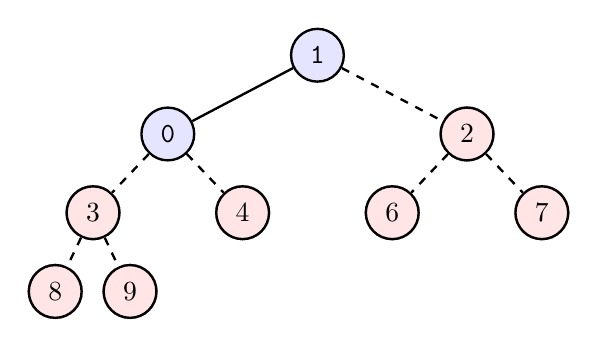
\begin{tikzpicture}

\fill[blue!10] (0.0, 0.0) circle (0.35);
\node [line width=0.03cm,black,minimum size=0.6699999999999999cm,draw,circle] at (0.0,0.0)(1){};\draw (0.0, 0.0) node[color=black] {\texttt{1}};
\fill[blue!10] (-1.9, -1.0) circle (0.35);
\node [line width=0.03cm,black,minimum size=0.6699999999999999cm,draw,circle] at (-1.9,-1.0)(0){};\draw (-1.9, -1.0) node[color=black] {\texttt{0}};
\fill[blue!10] (1.9, -1.0) circle (0.35);
\node [line width=0.03cm,black,minimum size=0.6699999999999999cm,draw,circle] at (1.9,-1.0)(2){};\draw (1.9, -1.0) node[color=black] {\texttt{2}};
\fill[blue!10] (-2.85, -2.0) circle (0.35);
\node [line width=0.03cm,black,minimum size=0.6699999999999999cm,draw,circle] at (-2.85,-2.0)(3){};\draw (-2.85, -2.0) node[color=black] {\texttt{3}};
\fill[blue!10] (-0.95, -2.0) circle (0.35);
\node [line width=0.03cm,black,minimum size=0.6699999999999999cm,draw,circle] at (-0.95,-2.0)(4){};\draw (-0.95, -2.0) node[color=black] {\texttt{4}};
\fill[blue!10] (0.95, -2.0) circle (0.35);
\node [line width=0.03cm,black,minimum size=0.6699999999999999cm,draw,circle] at (0.95,-2.0)(6){};\draw (0.95, -2.0) node[color=black] {\texttt{6}};
\fill[blue!10] (2.85, -2.0) circle (0.35);
\node [line width=0.03cm,black,minimum size=0.6699999999999999cm,draw,circle] at (2.85,-2.0)(7){};\draw (2.85, -2.0) node[color=black] {\texttt{7}};
\fill[blue!10] (-3.33, -3.0) circle (0.35);
\node [line width=0.03cm,black,minimum size=0.6699999999999999cm,draw,circle] at (-3.33,-3.0)(8){};\draw (-3.33, -3.0) node[color=black] {\texttt{8}};
\fill[blue!10] (-2.38, -3.0) circle (0.35);
\node [line width=0.03cm,black,minimum size=0.6699999999999999cm,draw,circle] at (-2.38,-3.0)(9){};\draw (-2.38, -3.0) node[color=black] {\texttt{9}};\draw[line width=0.03cm,black] (1) to  (0);
\draw[line width=0.03cm,black] (1) to  (2);
\draw[line width=0.03cm,black] (0) to  (3);
\draw[line width=0.03cm,black] (0) to  (4);
\draw[line width=0.03cm,black] (2) to  (6);
\draw[line width=0.03cm,black] (2) to  (7);
\draw[line width=0.03cm,black] (3) to  (8);
\draw[line width=0.03cm,black] (3) to  (9);

\fill[red!10] (-2.38, -3.0) circle (0.35);
\draw[line width=0.03cm,black] (-2.38, -3.0) circle (0.33499999999999996);\draw (-2.38, -3.0) node[color=black] {9};
\fill[red!10] (-3.33, -3.0) circle (0.35);
\draw[line width=0.03cm,black] (-3.33, -3.0) circle (0.33499999999999996);\draw (-3.33, -3.0) node[color=black] {8};
\fill[red!10] (2.85, -2.0) circle (0.35);
\draw[line width=0.03cm,black] (2.85, -2.0) circle (0.33499999999999996);\draw (2.85, -2.0) node[color=black] {7};
\fill[red!10] (0.95, -2.0) circle (0.35);
\draw[line width=0.03cm,black] (0.95, -2.0) circle (0.33499999999999996);\draw (0.95, -2.0) node[color=black] {6};
\fill[red!10] (-0.95, -2.0) circle (0.35);
\draw[line width=0.03cm,black] (-0.95, -2.0) circle (0.33499999999999996);\draw (-0.95, -2.0) node[color=black] {4};
\fill[red!10] (-2.85, -2.0) circle (0.35);
\draw[line width=0.03cm,black] (-2.85, -2.0) circle (0.33499999999999996);\draw (-2.85, -2.0) node[color=black] {3};
\fill[red!10] (1.9, -1.0) circle (0.35);
\draw[line width=0.03cm,black] (1.9, -1.0) circle (0.33499999999999996);\draw (1.9, -1.0) node[color=black] {2};\draw[line width=0.1cm,white] (1) to  (2);
\draw[line width=0.03cm,black,,dashed] (1) to  (2);
\draw[line width=0.1cm,white] (3) to  (9);
\draw[line width=0.03cm,black,,dashed] (3) to  (9);
\draw[line width=0.1cm,white] (3) to  (8);
\draw[line width=0.03cm,black,,dashed] (3) to  (8);
\draw[line width=0.1cm,white] (2) to  (7);
\draw[line width=0.03cm,black,,dashed] (2) to  (7);
\draw[line width=0.1cm,white] (2) to  (6);
\draw[line width=0.03cm,black,,dashed] (2) to  (6);
\draw[line width=0.1cm,white] (0) to  (4);
\draw[line width=0.03cm,black,,dashed] (0) to  (4);
\draw[line width=0.1cm,white] (0) to  (3);
\draw[line width=0.03cm,black,,dashed] (0) to  (3);
\end{tikzpicture}

\end{center}


\begin{center}
\begin{tikzpicture}

\fill[white] (0.0, 0.0) circle (0.3);
\node [line width=0.03cm,black,minimum size=0.57cm,draw,circle] at (0.0,0.0)(10){};\draw (0.0, 0.0) node[color=black] {\texttt{10}};
\fill[white] (-3.0, -1.0) circle (0.35);
\node [line width=0.1cm,red,minimum size=0.6cm,draw,circle] at (-3.0,-1.0)(5){};\draw (-3.0, -1.0) node[color=black] {\texttt{5}};
\fill[white] (3.0, -1.0) circle (0.3);
\node [line width=0.03cm,black,minimum size=0.57cm,draw,circle] at (3.0,-1.0)(18){};\draw (3.0, -1.0) node[color=black] {\texttt{18}};
\fill[white] (-4.5, -2.0) circle (0.3);
\node [line width=0.03cm,black,minimum size=0.57cm,draw,circle] at (-4.5,-2.0)(2){};\draw (-4.5, -2.0) node[color=black] {\texttt{2}};
\fill[white] (-5.25, -3.0) circle (0.3);
\node [line width=0.03cm,black,minimum size=0.57cm,draw,circle] at (-5.25,-3.0)(0){};\draw (-5.25, -3.0) node[color=black] {\texttt{0}};\draw[line width=0.03cm,black,->,>=triangle 60] (10) to  (5);
\draw[line width=0.03cm,black,->,>=triangle 60] (10) to  (18);
\draw[line width=0.1cm,red,->,>=triangle 60] (5) to  (2);
\draw[line width=0.1cm,red,->,>=triangle 60] (2) to  (0);
\end{tikzpicture}

\end{center}




\textsc{Step 8}.
I swap \texttt{1} and \texttt{0}

\begin{center}
\begin{tikzpicture}

\fill[white] (0.0, 0.0) circle (0.3);
\node [line width=0.03cm,black,minimum size=0.57cm,draw,circle] at (0.0,0.0)(10){};\draw (0.0, 0.0) node[color=black] {\texttt{10}};
\fill[white] (-1.5, -1.0) circle (0.35);
\node [line width=0.1cm,red,minimum size=0.6cm,draw,circle] at (-1.5,-1.0)(2){};\draw (-1.5, -1.0) node[color=black] {\texttt{2}};
\fill[white] (1.5, -1.0) circle (0.3);
\node [line width=0.03cm,black,minimum size=0.57cm,draw,circle] at (1.5,-1.0)(18){};\draw (1.5, -1.0) node[color=black] {\texttt{18}};
\fill[white] (-2.25, -2.0) circle (0.3);
\node [line width=0.03cm,black,minimum size=0.57cm,draw,circle] at (-2.25,-2.0)(0){};\draw (-2.25, -2.0) node[color=black] {\texttt{0}};
\fill[white] (-0.75, -2.0) circle (0.3);
\node [line width=0.03cm,black,minimum size=0.57cm,draw,circle] at (-0.75,-2.0)(5){};\draw (-0.75, -2.0) node[color=black] {\texttt{5}};\draw[line width=0.03cm,black,->,>=triangle 60] (10) to  (2);
\draw[line width=0.03cm,black,->,>=triangle 60] (10) to  (18);
\draw[line width=0.03cm,black,->,>=triangle 60] (2) to  (0);
\draw[line width=0.03cm,black,->,>=triangle 60] (2) to  (5);
\end{tikzpicture}

\end{center}



Clearly there's no need to heapify-down since the tree now has size 1.
At this point, the array is
\begin{center}
\begin{tikzpicture}

\fill[white] (0.0, 0.0) circle (0.3);
\node [line width=0.03cm,black,minimum size=0.57cm,draw,circle] at (0.0,0.0)(10){};\draw (0.0, 0.0) node[color=black] {\texttt{10}};
\fill[white] (-3.0, -1.0) circle (0.3);
\node [line width=0.03cm,black,minimum size=0.57cm,draw,circle] at (-3.0,-1.0)(2){};\draw (-3.0, -1.0) node[color=black] {\texttt{2}};
\fill[white] (3.0, -1.0) circle (0.3);
\node [line width=0.03cm,black,minimum size=0.57cm,draw,circle] at (3.0,-1.0)(18){};\draw (3.0, -1.0) node[color=black] {\texttt{18}};
\fill[white] (-4.5, -2.0) circle (0.3);
\node [line width=0.03cm,black,minimum size=0.57cm,draw,circle] at (-4.5,-2.0)(0){};\draw (-4.5, -2.0) node[color=black] {\texttt{0}};
\fill[white] (-1.5, -2.0) circle (0.3);
\node [line width=0.03cm,black,minimum size=0.57cm,draw,circle] at (-1.5,-2.0)(5){};\draw (-1.5, -2.0) node[color=black] {\texttt{5}};
\fill[white] (-2.25, -3.0) circle (0.3);
\node [line width=0.03cm,black,minimum size=0.57cm,draw,circle] at (-2.25,-3.0)(3){};\draw (-2.25, -3.0) node[color=black] {\texttt{3}};\draw[line width=0.1cm,red,->,>=triangle 60] (10) to  (2);
\draw[line width=0.03cm,black,->,>=triangle 60] (10) to  (18);
\draw[line width=0.03cm,black,->,>=triangle 60] (2) to  (0);
\draw[line width=0.1cm,red,->,>=triangle 60] (2) to  (5);
\draw[line width=0.1cm,red,->,>=triangle 60] (5) to  (3);
\end{tikzpicture}

\end{center}


It's sorted!

Here's the algorithm:
\begin{console}
ALGORITHM: heapsort
INPUT:     x - array
           n - length of x

Perform build_maxheap on x[0..n - 1]
for i = n - 1, n - 2, ..., 1: 
    swap x[0] and x[i]
    perform heapify_down on x[0..i - 1] at index 0
\end{console}


\begin{ex} 
  \label{ex:some-decision1}
  \tinysidebar{\debug{exercises/{empty0/question.tex}}}
  \solutionlink{sol:some-decision1}
  \qed
\end{ex} 
\begin{python0}
from solutions import *
add(label="ex:some-decision1",
    srcfilename='exercises/some-decision1/answer.tex') 
\end{python0}



\begin{ex} 
  \label{ex:some-decision1}
  \tinysidebar{\debug{exercises/{empty0/question.tex}}}
  \solutionlink{sol:some-decision1}
  \qed
\end{ex} 
\begin{python0}
from solutions import *
add(label="ex:some-decision1",
    srcfilename='exercises/some-decision1/answer.tex') 
\end{python0}



\begin{ex} 
  \label{ex:some-decision1}
  \tinysidebar{\debug{exercises/{empty0/question.tex}}}
  \solutionlink{sol:some-decision1}
  \qed
\end{ex} 
\begin{python0}
from solutions import *
add(label="ex:some-decision1",
    srcfilename='exercises/some-decision1/answer.tex') 
\end{python0}

% The minimum must be a leave. Look at $n/2, ..., n - 1$.
% n-1 - n/2 + 1 = n - n / 2 accesses.


\begin{ex} 
  \label{ex:some-decision1}
  \tinysidebar{\debug{exercises/{empty0/question.tex}}}
  \solutionlink{sol:some-decision1}
  \qed
\end{ex} 
\begin{python0}
from solutions import *
add(label="ex:some-decision1",
    srcfilename='exercises/some-decision1/answer.tex') 
\end{python0}

